\section{Sensor Fusion for Self-Balancing Robot using MPU6050}
\subsection{Introduction}
Self-balancing robots require accurate estimation of their tilt angle for effective control. The MPU6050, a widely used Inertial Measurement Unit (IMU), provides raw accelerometer and gyroscope data. However, due to individual sensor limitations, direct usage of these readings is unreliable. Sensor fusion techniques like the Complementary Filter and Kalman Filter help in obtaining a stable and accurate tilt angle

\subsubsection{Microcontroller}
The ATmega328P (shown in Fig. \ref{fig:ATmega328p}) is a popular microcontroller from Microchip Technology, widely used in embedded systems and electronics projects. With a 16 MHz clock speed, 32 KB of flash memory, 2 KB of SRAM, and 1 KB of EEPROM \cite{atmega_microchip}, the ATmega328P provides ample resources for this projects application. 

The ATMEGA328P is also used in the Arduino Nano (shown in Fig. \ref{fig:arduino_nano}), a widely adopted development board known for its low cost and open-source ecosystem \cite{arduino_nano}. The combination of affordability and extensive community support makes it an ideal choice for rapid prototyping and academic research, ensuring easy integration with various sensors and motor drivers. 

\begin{figure}[H]
	\centering
	\subfloat[ATMEGA328P \cite{atmega_microchip}.]{
		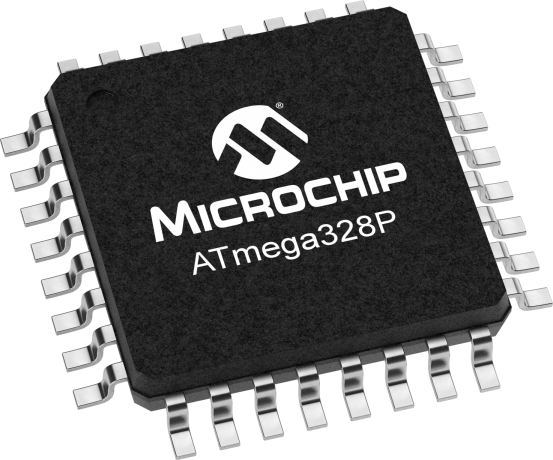
\includegraphics[height=3cm]{assets/ATmega328p.png}
		\label{fig:ATmega328p}
	}
	\qquad
	\subfloat[Arduino Nano \cite{arduino_nano}.]{
	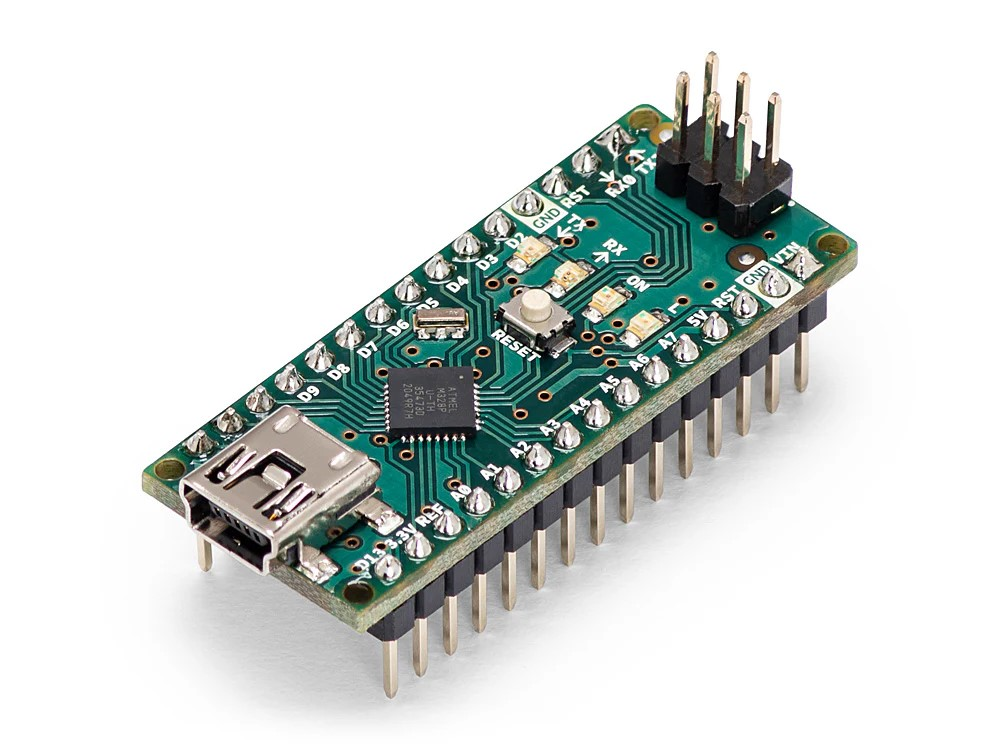
\includegraphics[height=3cm]{assets/arduino_nano.jpg}
	\label{fig:arduino_nano}
	} 
	\label{fig:ATmega328p_and_arduino_nano}
	\caption{}
\end{figure}

\subsubsection{Inertial Measuring Unit}
The MPU6050 is a widely used six-axis sensor that integrates a three-axis gyroscope and a three-axis accelerometer on a single chip, making it essential for motion tracking and stabilization applications (shown in Fig. \ref{fig:mpu-6050}). Its compact design and built-in Digital Motion Processor (DMP) enable real-time processing of sensor data, which is crucial for robotics, drones, and wearable devices.
In applications like self-balancing robots, it provides accurate orientation and acceleration data necessary for maintaining stability. 

\begin{figure}[H]
	\centering
	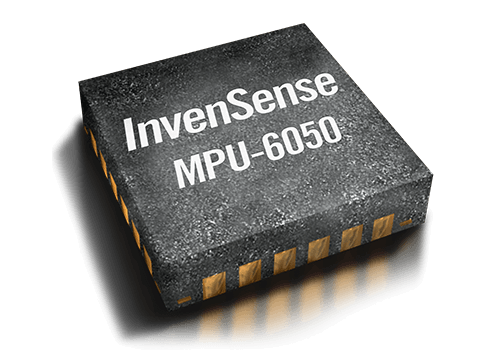
\includegraphics[height=3cm]{assets/mpu-6050.png}
	\caption{MPU-6050 \cite{mpu6050}.}
	\label{fig:mpu-6050}
\end{figure}


\subsection{Working of MPU6050}
The MPU6050 is a 6-axis IMU that provides:
\begin{itemize}
	\item Accelerometer Data: Measures acceleration in X, Y, and Z axes. It helps in estimating tilt based on gravitational force.
	\item Gyroscope Data: Measures angular velocity around X, Y, and Z axes. Integration of gyroscope readings over time provides the tilt angle.
\end{itemize}

\subsubsection{Reading Raw Sensor Data}
The \texttt{read\_mpu\_6050\_data()} function reads raw data from the MPU6050 sensor:
\begin{itemize}
	\item It requests 14 bytes of data from the sensor, covering the accelerometer, gyroscope, and temperature sensor readings.
	\item The data is stored in respective variables after combining the high and low bytes. 
	\item If data retrieval fails, an error message is displayed.
\end{itemize}
\begin{lstlisting}[style=cppstyle2]
void mpu6050Base::read_mpu_6050_data() {
	Wire.beginTransmission(mpu6050_addr);
	Wire.write(0x3B);
	Wire.endTransmission();
	Wire.requestFrom(mpu6050_addr, (uint8_t)14);
	
	if (Wire.available() >= 14) {
		acc_x = Wire.read() << 8 | Wire.read();
		acc_y = Wire.read() << 8 | Wire.read();
		acc_z = Wire.read() << 8 | Wire.read();
		temperature = Wire.read() << 8 | Wire.read();
		gyro_x = Wire.read() << 8 | Wire.read();
		gyro_y = Wire.read() << 8 | Wire.read();
		gyro_z = Wire.read() << 8 | Wire.read();
	} else {
		ERROR_PRINT("Data cannot be read from MPU6050!");
	}
	
}
\end{lstlisting}

\subsubsection{Issues with Raw Sensor Data}
\begin{itemize}
\item \textbf{Accelerometer Noise}: While providing an absolute angle reference, accelerometer readings are noisy and susceptible to external forces.
\item \textbf{Gyroscope Drift}: Over time, integration errors cause drift, leading to inaccurate angle estimation.
To overcome these issues, sensor fusion techniques are applied.
\end{itemize}


\subsection{Complementary Filter}
The complementary filter is a simple yet effective method for sensor fusion \cite{rabbany_design_2021} \cite{10193276} \cite{1174486}. It blends high-frequency data from the gyroscope with low-frequency data from the accelerometer:

\subsubsection{Mathematical Model}
Raw accelerometer readings $A_y$ and $Az$ can be used to calculate tilt angle using following equation:
\begin{equation}
\theta_{acc} = \text{arctan} \left(A_y/Az  \right) \label{eq:eq}
\end{equation}
Similarly, using raw angular velocity data from the gyroscope $\omega_{x}$,
\begin{equation}
	\begin{aligned}
		\dot{\theta}_{gyro}(t) &= - \omega_{x,bias}(t) \\ \label{eq:state_eq_1}
		\dot{\omega}_{x,bias}(t) &= 0
	\end{aligned}
\end{equation}
In these equations, $\theta(t)$ represents the measured angle of the system, and $\omega_{\text{gyro,bias}}(t)$ represents the bias of the gyroscope. The first equation models how the angle evolves over time, influenced by the constant gyroscope bias. The second equation indicates that the gyroscope bias remains constant over time. The sampling time interval $\Delta t$ and previous angle value $\theta_{previous}$ can be used to calculate tilt angle using following equation:
\begin{equation}
\theta_{gyro} = \theta_{previous, gyro} + \omega_{gyro} \Delta t \label{eq:eq}
\end{equation}
Then the final estimated angle $\theta_{estimate}$ is calculated as:
\begin{equation}
	\theta_{estimate} = \alpha \ \theta_{gyro} + (1 - \alpha) \ \theta_{acc} \label{eq:eq}
\end{equation}
Where $\alpha$ is the filter coefficient, $\omega$ is the angular velocity from the gyroscope, and $\theta_{acc}$ is the angle from the accelerometer.

\subsubsection{Initial Calibration}
The \texttt{init()} function is responsible for initializing the MPU6050 sensor and performing gyroscope calibration:
\begin{itemize}
	\item The I2C communication is established with the sensor, and an acknowledgment is checked to ensure proper connection.
	\item The function sets up the MPU6050 registers using \texttt{setup\_mpu\_6050\_registers()}, configuring the power management and sensitivity ranges for both the accelerometer and gyroscope.
	\item Gyroscope calibration is performed by collecting multiple readings and averaging them to calculate offsets for the X, Y, and Z axes. These offsets help reduce sensor drift.
\end{itemize}

\begin{lstlisting}[style=cppstyle2]
void mpu6050Base::init() {
	Wire.beginTransmission(mpu6050_addr);
	if (Wire.endTransmission() != 0) {
		ERROR_PRINT("MPU6050 not connected!");
		return;
	}
	setup_mpu_6050_registers();
	
	for (int i = 0; i < CALIBRATION_SAMPLES; i++) {
		read_mpu_6050_data();
		gyro_x_cal += gyro_x;
		gyro_y_cal += gyro_y;
		gyro_z_cal += gyro_z;
		delay(3);
	}
	gyro_x_cal /= CALIBRATION_SAMPLES;
	gyro_y_cal /= CALIBRATION_SAMPLES;
	gyro_z_cal /= CALIBRATION_SAMPLES;
}
\end{lstlisting}

\subsubsection{Calculating Angles}
The \texttt{calculate()} function processes raw sensor data to determine pitch and roll angles:
\begin{itemize}
	\item Gyroscope readings are corrected using calibration offsets to remove bias.
	\item Angular velocity is integrated over time to estimate orientation changes.
	\item The accelerometer-derived angles are computed from the total acceleration vector using trigonometric transformations.
	\item A complementary filter is applied to blend gyroscope and accelerometer readings, mitigating drift and noise while enhancing stability.
\end{itemize}

\begin{lstlisting}[style=cppstyle2]
void mpu6050Base::calculate() {
	read_mpu_6050_data();
	
	gyro_x -= gyro_x_cal;
	gyro_y -= gyro_y_cal;
	gyro_z -= gyro_z_cal;
	
	angle_pitch += gyro_x * 0.0000611;
	angle_roll += gyro_y * 0.0000611;
	
	angle_pitch += angle_roll * sin(gyro_z * 0.000001066);
	angle_roll -= angle_pitch * sin(gyro_z * 0.000001066);
	
	acc_total_vector = sqrt((acc_x * acc_x) + (acc_y * acc_y) + (acc_z * acc_z));
	
	angle_pitch_acc = asin((float)acc_y / acc_total_vector) * 57.296;
	angle_roll_acc = asin((float)acc_x / acc_total_vector) * -57.296;
	
	if (set_gyro_angles) {
		angle_pitch = angle_pitch * 0.9996 + angle_pitch_acc * 0.0004;
		angle_roll = angle_roll * 0.9996 + angle_roll_acc * 0.0004;
	} else {
		angle_pitch = angle_pitch_acc;
		angle_roll = angle_roll_acc;
		set_gyro_angles = true;
	}
	
	angle_pitch_output = angle_pitch_output * 0.9 + angle_pitch * 0.1;
	angle_roll_output = angle_roll_output * 0.9 + angle_roll * 0.1;
	
}
\end{lstlisting}


\subsubsection{Results}

\begin{figure}[H]
	\centering
	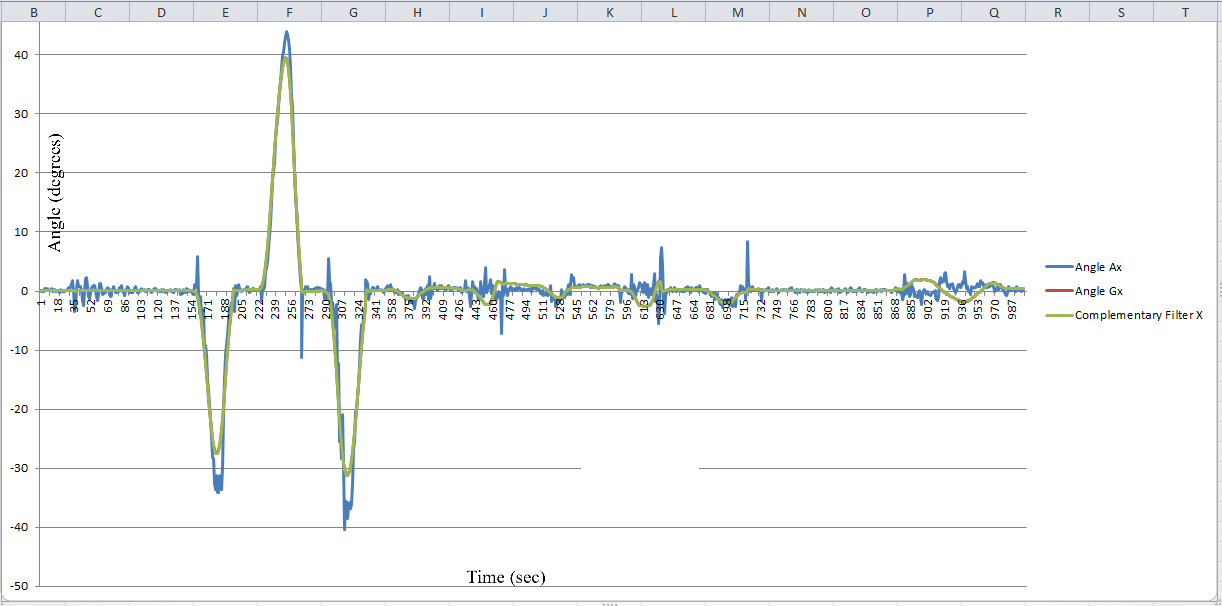
\includegraphics[height=8cm]{assets/compl_filter_0.9.png}
	\caption{Pitch angle caluclated using a complementary filter with $\omega = 0.9$.}
	\label{fig:battery}
\end{figure}
